\begin{answer}
Notice, if
$$
\begin{aligned}
\frac{h(x^{(i)})}{\alpha} &= \frac{1}{2}\\
\therefore \frac{1}{1+\exp(-\theta_\text{new}^Tx)} &= \frac{\alpha}{2}\\
\theta_\text{new}^Tx = \theta^{\text{new}}_0 + \theta^{\text{new}}_1x_1 + \theta^{\text{new}}_2x_2&= - \log(\frac{2}{\alpha}-1)\\
\end{aligned}
$$
We can see that,
$$
\theta^\text{new}_0 =\theta^\text{old}_0 \underbrace{ (1+\log(\frac{2}{\alpha}-1))}_\text{correction factor in the question}
$$
\begin{figure}[htbp]
    \begin{subfigure}[b]{0.3\linewidth}
        \centering
        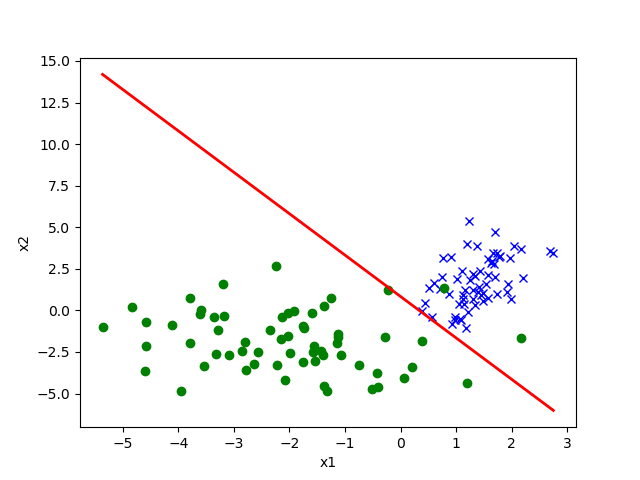
\includegraphics[width=\linewidth]{pics/p02c.png}
        \caption{Train on t}
    \end{subfigure}
    \begin{subfigure}[b]{0.3\linewidth}
        \centering
        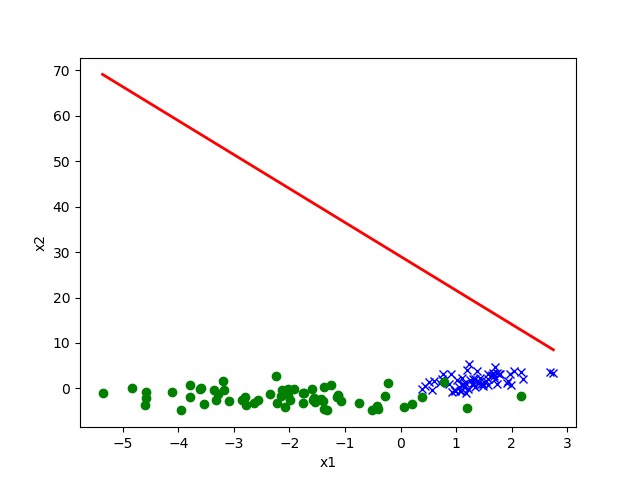
\includegraphics[width=\linewidth]{pics/p02d.png}
        \caption{Train on y}
    \end{subfigure}
    \begin{subfigure}[b]{0.3\linewidth}
        \centering
        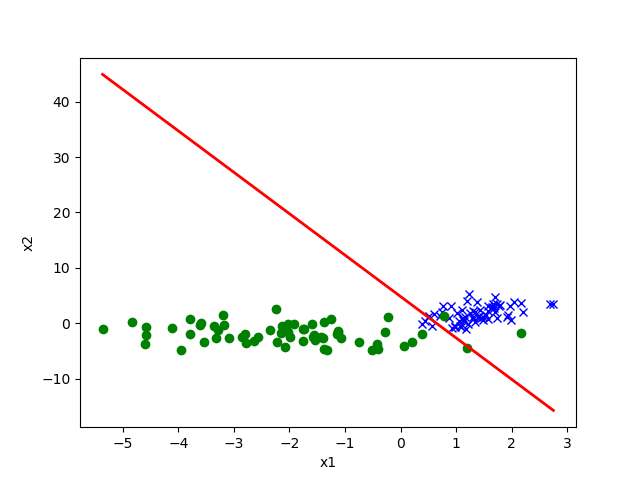
\includegraphics[width=\linewidth]{pics/p02e.png}
        \caption{Train on t, with rescale}
    \end{subfigure}

\end{figure}
\end{answer}
